\documentclass[border=10pt]{standalone}
\usepackage{pgfplots}
\usepgfplotslibrary{fillbetween}
\pgfplotsset{compat=1.18}
\begin{document}
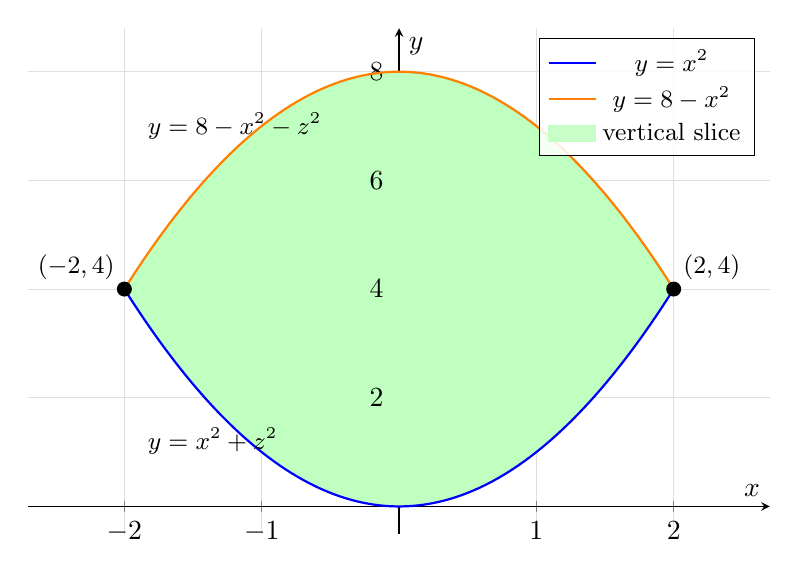
\begin{tikzpicture}
\begin{axis}[
    axis lines=middle,
    xlabel=$x$, ylabel=$y$,
    xmin=-2.7, xmax=2.7,
    ymin=-0.5, ymax=8.8,
    width=11cm, height=8cm,
    grid=both,
    grid style={gray!25},
    legend style={font=\small, at={(0.98,0.98)}, anchor=north east, fill=white, fill opacity=0.85, text opacity=1}
]
\addplot[name path=A, blue, thick, domain=-2:2, samples=100] {x^2};
\addlegendentry{$y=x^2$}
\addplot[name path=B, orange, thick, domain=-2:2, samples=100] {8-x^2};
\addlegendentry{$y=8-x^2$}
\addplot[green!25] fill between[of=A and B];
\addlegendentry{vertical slice}
\addplot[only marks, mark=*, mark size=2.5pt, black] coordinates {(-2,4) (2,4)};
\node[above left, font=\small] at (axis cs:-2,4) {$(-2,4)$};
\node[above right, font=\small] at (axis cs:2,4) {$(2,4)$};
\node[font=\small, anchor=west] at (axis cs:-1.9,1.2) {$y=x^2+z^2$};
\node[font=\small, anchor=west] at (axis cs:-1.9,7.0) {$y=8-x^2-z^2$};
\end{axis}
\end{tikzpicture}
\end{document}